%----------------------------------------------------------------------------------------------------------
% 	Copyright (c) 2009 R-forge 'distributions' Core Team, 
% 	
%	The following Sweave code is under the GNU Free Documentation License:
%      	Permission is granted to copy, distribute and/or modify this document
%      	under the terms of the GNU Free Documentation License, Version 1.3
%      	or any later version published by the Free Software Foundation;
%      	with no Invariant Sections, no Front-Cover Texts, and no Back-Cover Texts.
%
%      A copy of the license is included in the 'inst' directory of this package 
%      or on the web at http://www.gnu.org/licenses/licenses.html#FDL
%
%	After running Sweave, the following code could be compiled :
%	  - on windows with a Tex distribution such as miktex (http://miktex.org) 
%		and a front end Latex editor such as texniccenter (http://www.toolscenter.org)
%	  - on mac os with a Tex distribution such as TexLive and a front end Latex
%	  	editor such as Texshop (http://www.uoregon.edu/~koch/texshop/)
%	  - on linux with a Tex distribution such as teTex (http://www.tug.org/teTeX/)
%	  	and a front end Latex editor such as emacs (http://www.gnu.org/software/emacs/)
%
%----------------------------------------------------------------------------------------------------------

\chapter{Student and related distributions}
%%%%%%%%%%%%%%%%%%%%%%%%%%%%%%%%%%%%%%%%%%%%%
\section{Student t distribution}
Intro?
\subsection{Characterization}
\begin{wrapfigure}{r}{0.5\textwidth}
  \vspace{-20pt}
  \begin{center}
    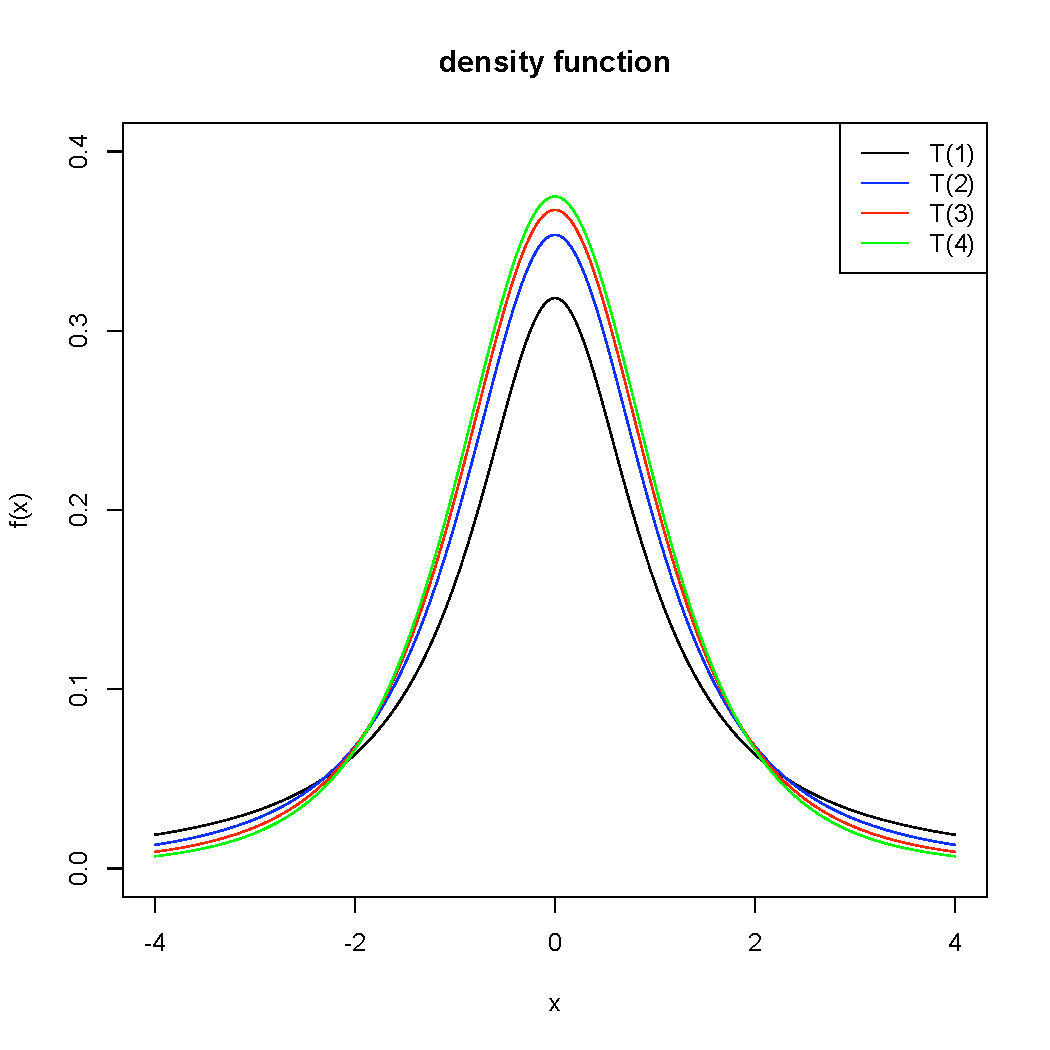
\includegraphics[width=0.48\textwidth]{img/studentzoom}
  \end{center}
  \vspace{-20pt}  
  \caption{Density function for student distributions}
%  \vspace{-20pt}  
\end{wrapfigure}

There are many ways to define the student distribution. One can say that it is the distribution of
$$
\frac{\sqrt{d}N}{C},
$$
where $N$ is a standard normal variable independent of $C$ a chi-squared variable with $d$ degrees of freedom. We can derive the following density function
$$
f(x) =  \frac{\Gamma(\frac{d+1}{2})}{\sqrt{\pi d} \Gamma(\frac{d}{2}) } \left(1+\frac{x^2}{d}\right)^{-\frac{d+1}{2}},
$$
for $x\in\mbb R$. $d$ is not necessarily an integer, it could be a real but greater than 1.

The distribution function of the student t distribution is given by
$$
F(x) = \frac{1}{2} + x \Gamma \left( \frac{d+1}{2} \right) \frac{ \,_2F_1 \left ( \frac{1}{2},\frac{d+1}{2};\frac{3}{2}; -\frac{x^2}{d} \right)}   {\sqrt{\pi\nu}\,\Gamma (\frac{d}{2})},
$$
where $\,_2F_1$ denotes the hypergeometric function.

\subsection{Properties}
The expectation of a student distribution is $E(X)=0$ if $d>1$, infinite otherwise. And the variance is given by $Var(X) = \frac{d}{d-2}$ if $d>2$.

Moments are given by
$$
E(X^r) = \prod_{i=1}^{r/2} \frac{2i-1}{\nu - 2i}\nu^{r/2},
$$
where $r$ is an even integer.

\subsection{Estimation}
Maximum likelihood estimator for $d$ can be found by solving numerically this equation
$$
\psi\left ( \frac{d+1}{2}\right) - \psi\left ( \frac{d}{2}\right) = \frac{1}{n}\sum_{i=1}^n\log\left(1+\frac{X_i^2}{d}\right) - \frac{d+1}{n} \sum_{i=1}^n \frac{(X_i/d)^2}{1+X_i^2/d},
$$
where $\psi$ denotes the digamma function.

\subsection{Random generation}
The algorithm is simply
\begin{itemize}
\item generate a standard normal distribution $N$
\item generate a chi-squared distribution $C$
\item return $\frac{\sqrt{d}N}{\sqrt{C}}$.
\end{itemize}

\subsection{Applications}
The main application of the student is when dealing with a normally distributed sample, the derivation of the  confidence interval for the standard deviation use the student distribution. Indeed for a normally distributed $\mcal N(m,\sigma^2)$ sample of size $n$ we have that  
$$
\frac{\bar X_n-m}{\sqrt{S_n^2}}\sqrt{n}
$$ 
follows a student $n$ distribution.

%%%%%%%%%%%%%%%%%%%%%%%%%%%%%%%%%%%%%%%%%%%%%
\section{Cauchy distribution}
\subsection{Characterization}
\subsection{Characterization}
\begin{wrapfigure}{r}{0.5\textwidth}
  \vspace{-20pt}
  \begin{center}
    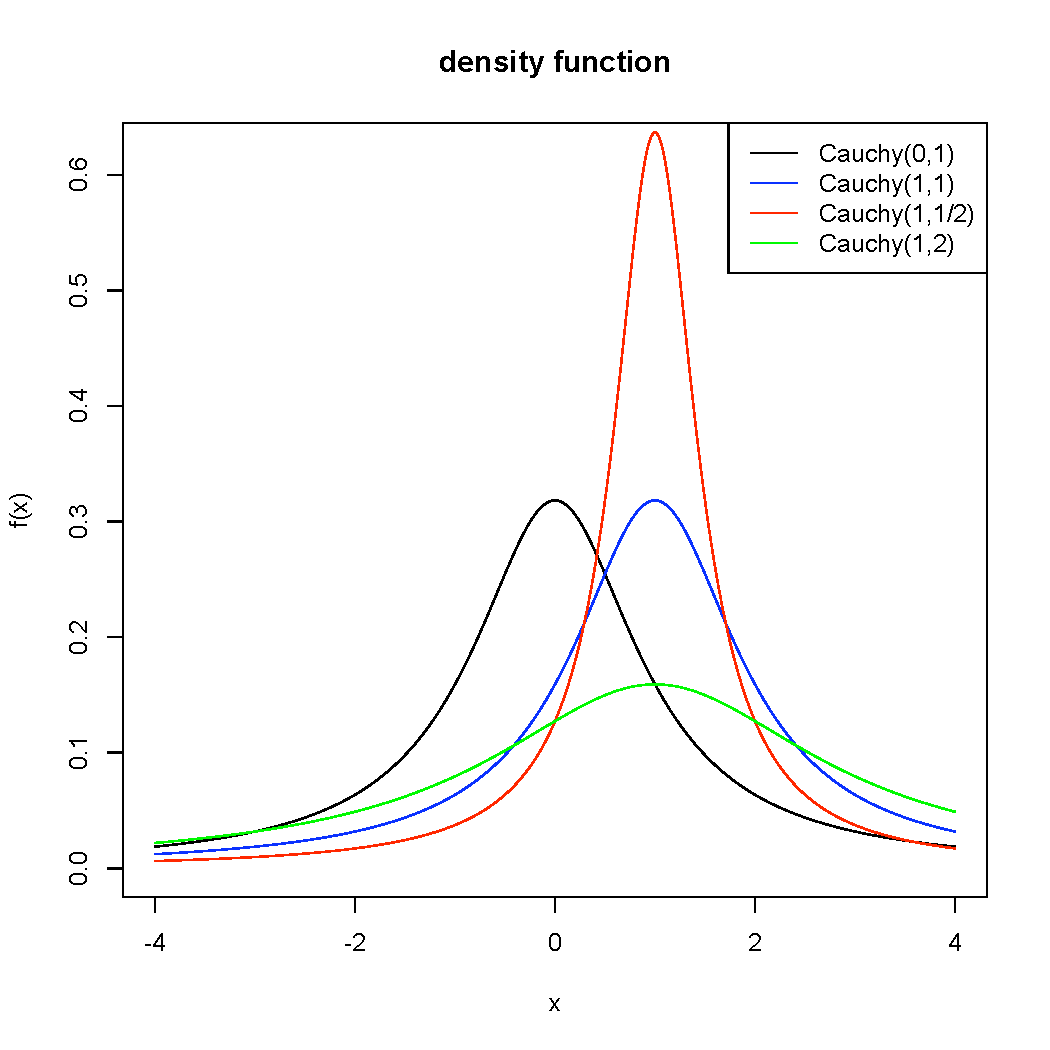
\includegraphics[width=0.48\textwidth]{img/cauchyzoom}
  \end{center}
  \vspace{-20pt}  
  \caption{Density function for Cauchy distributions}
%  \vspace{-20pt}  
\end{wrapfigure}
The Cauchy distribution is a special case of the Student distribution when a degree of freedom of $1$. Therefore the density function is
$$
f(x) =\frac{1}{\pi(1+x^2)},
$$
where $x\in \mathbb R$. Its distribution function is 
$$
F(x) = \frac{1}{\pi} \arctan(x)+\frac{1}{2}.
$$

There exists a scaled and shifted version of the Cauchy distribution coming from the scaled and shifted version of the student distribution. The density is
$$
f(x) = \frac{\gamma^2}{\pi \left[\gamma^2 + (x-\delta)^2\right]},
$$
while its distribution function is 
$$
F(x) = \frac{1}{\pi} \arctan\left(\frac{x-\delta}{\gamma}\right)+\frac{1}{2}.
$$
Even if there is no moment generating function, the Cauchy distribution has a characteristic function
$$
\phi(t) = \exp(\delta\,i\,t-\gamma\,|t|).
$$


\subsection{Properties}
The Cauchy distribution $\mathcal C(\delta, \gamma)$ has the horrible feature not to have any finite moments. However, the Cauchy distribution belongs to the family of stable distribution, thus a sum of Cauchy distribution is still a Cauchy distribution.

\subsection{Estimation}
Maximum likelihood estimators verify the following system
$$
\left\{
\begin{array}{l}
\frac{1}{\gamma} = \frac{1}{n} \sum\limits_{i=1}^n\frac{\gamma}{\gamma^2+(X_i-\delta)^2}\\
\sum\limits_{i=1}^n\frac{X_i}{\gamma^2+(X_i-\delta)^2} = \sum\limits_{i=1}^n\frac{\delta}{\gamma^2+(X_i-\delta)^2}\\
\end{array}
\right. .
$$
There is no moment based estimators.

\subsection{Random generation}
Since the quantile function is $F^{-1}(u) = \delta+\gamma\tan((u-1/2)\pi)$, we can use the inversion function method.

\subsection{Applications}
NEED REFERENCE


%%%%%%%%%%%%%%%%%%%%%%%%%%%%%%%%%%%%%%%%%%%%
\section{Fisher-Snedecor distribution}
\subsection{Characterization}
TODO
\subsection{Properties}
TODO
\subsection{Estimation}
TODO
\subsection{Random generation}
TODO
\subsection{Applications}
TODO